\subsection{Математическое ожидание и дисперсия}

    На графике \ref{EV_cyclic} прелставлены зависимости математического ожидания и дисперсии системы \(\ref{beta_chaos}\) для \(\beta\)-шума. В зависимости от параметра \(\beta\) и интенсивности шума \(\varepsilon\). На графике зависимости математического ожидания хорошо видно уменьшение параметрического интервала выживаемости популяции при увеличении интенсивности шума. Далее данное явление будет описано с помощью функции Стохастической чувствительности.
        
    \begin{figure}
        \centering
        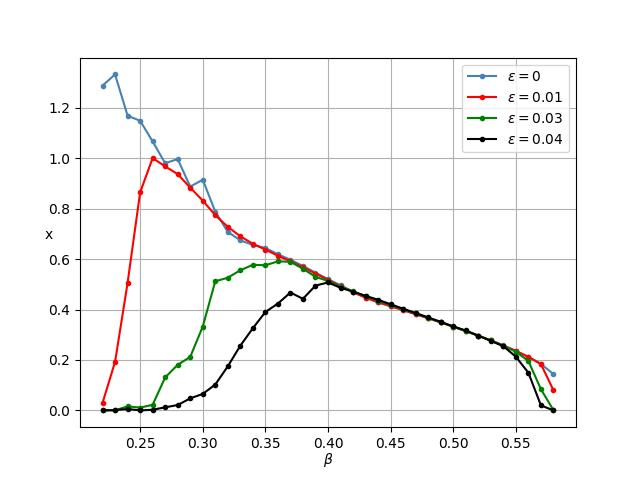
\includegraphics[width=\textwidth]{stochastic/images/EV_cyclic.jpg}
        
        \captionsetup{justification=centering}
        \caption{Усредненное математическое ожидание}
        \label{EV_cyclic}
    \end{figure}

    \begin{figure}
        \centering
        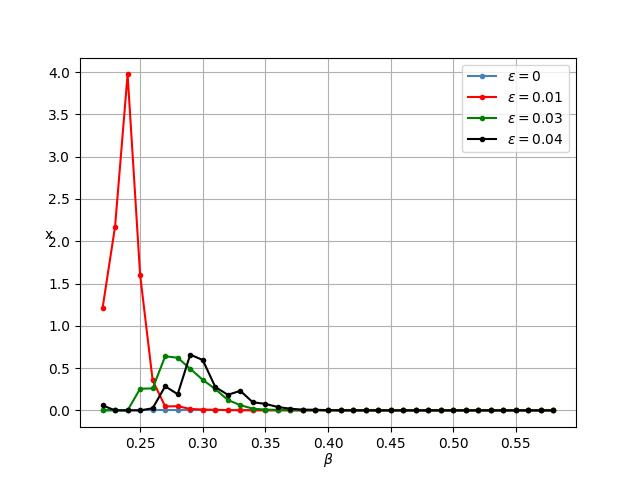
\includegraphics[width=\textwidth]{stochastic/images/variance_cyclic.jpg}
        
        \captionsetup{justification=centering}
        \caption{Дисперсия}
        \label{variance_cyclic}
    \end{figure}
